\documentclass[12pt, twosided]{report}  % type of Documents


%_____________________________________PACKAGES__________________________________
\usepackage[utf8]{inputenc} % input encoding [utf8]
\usepackage[english]{babel} % setting spell-check for English
\usepackage{geometry} % for page margins
\usepackage{fancyhdr} % for header and footer
\usepackage{url} % package to include urls
\usepackage{datetime} % For inserting date and time
\usepackage{graphicx} % For inserting graphics
\usepackage{float} % for accurate placement of figures and tables
\usepackage[labelfont=bf,textfont=bf]{caption} % for having the captions in bold
\usepackage{amsmath} %for equations
\usepackage[hidelinks]{hyperref} % for adding hyperlinks (withouht ugly boxes)
\usepackage{nomencl} % For Nomenclature 
\makenomenclature
\usepackage{amssymb} % symbols for nomenclature
\usepackage{etoolbox} % For Creating Categories in Nomenclature

%_______________________________________________________________________________


% PAGE GEOMETRY
\geometry{left=1cm,right=1cm,top=1cm,bottom=1cm,includeheadfoot}


%_____________________________HEADER AND FOOTER_______________________
\fancypagestyle{mypagestyle}{
\fancyhead{}
\fancyfoot{}
\fancyhead[L]{\rightmark}
\fancyhead[R]{SARS-CoV-2: An Analysis of Spread of Infection}
\fancyfoot[R]{\today}
\fancyfoot[C]{\thepage}
\fancyfoot[L]{Divyansh Chahar}
\renewcommand{\headrulewidth}{0pt}
\renewcommand{\footrulewidth}{0.8pt}
}
%_____________________________________________________________________


%% This code creates the groups
% -----------------------------------------
\renewcommand\nomgroup[1]{%
	\ifstrequal{#1}{A}{\item[\Large\bfseries{Greek Characters}]}{%
	\ifstrequal{#1}{B}{\vspace{10pt} \item[\Large\bfseries{Roman Characters}]}{%
	\ifstrequal{#1}{C}{\vspace{10pt} \item[\Large\bfseries{Acronyms}]}{}}}%
}
% -----------------------------------------


\pagestyle{mypagestyle} % For Header and Footer
\renewcommand\thesection{\arabic{section}} % Section Numbers Stating From 1
\renewcommand{\thefigure}{\thesection-\arabic{figure}} % to include section numbers in figures

%%%%%%%%%%%%%%%%%%%%%
% TITLE PAGE BEGINS %
%%%%%%%%%%%%%%%%%%%%%

\begin{document}
	\begin{titlepage}
		\newgeometry{a4paper,top=3cm,bottom=1cm,right=3cm,left=3cm} % Setting Page Dimensions
		\begin{center}
			{\LARGE \textbf{SARS-CoV-2}}\\
			
			\hrulefill
		
			\textbf{An Analysis of Spread of Infection} 
			
			\null
			
			Divyansh Chahar
			
			\vfill
			
			\href{https://www.linkedin.com/in/divyanshchahar/}{
\includegraphics[width=0.25\linewidth]{./images/icons/my_qrcode.eps}}
		
			\null
		
			\href{https://www.linkedin.com/in/divyanshchahar/}{
\includegraphics[width=0.025\linewidth]{./images/icons/linkedin_logo.eps}}
			\href{https://www.linkedin.com/in/divyanshchahar/}{https://www.linkedin.com/in/divyanshchahar/}
			
			\null
			
			\href{https://www.linkedin.com/in/divyanshchahar/}{
\includegraphics[width=0.025\linewidth]{./images/icons/github_mark.eps}}
			\href{https://github.com/divyanshchahar}{https://github.com/divyanshchahar}
			
			\vfill
			
			\today
			
		\end{center}
	\end{titlepage}

%%%%%%%%%%%%%%%%%%%
% TITLE PAGE ENDS %
%%%%%%%%%%%%%%%%%%%

\restoregeometry

\nomenclature[A]{$N$}{Total Population}
\nomenclature[A]{$t$}{Time in days}
\nomenclature[A]{$S_t$}{Individual Susceptible at time $t$}
\nomenclature[A]{$I_t$}{Individual Infected at time $t$}
\nomenclature[A]{$R_t$}{Individual Removed at time $t$}
\nomenclature[A]{$\overline{I}$}{Average Infected}
\nomenclature[A]{$R$}{Reproduction Number}
\nomenclature[A]{$A_n$}{Moving Average}
\nomenclature[A]{x}{Parameter Under Consideration}
\nomenclature[A]{$G_t$}{Growth Rate at time $t$}
\nomenclature[B]{$\beta$}{Diseaese Transmission Rate Constant}
\nomenclature[B]{$\gamma$}{Recovery Rate}

\printnomenclature

\pagebreak

\section{Introduction}
SARS-CoV-2 or Severe Acute Respiratory Syndrome related Coronavirs-2, is a virus that causes Covid-19, which is commonly known as Coronavirs. The virus originated in Wuhan, capital of Hubei Province of People's Republic of China, Covid-19 was classified as \textit{Pandemic} by World Health Organization on \textit{11-March-2020}. At the time of writing this report Coronavirus has infected infected 7360239 and killed 416201 individuals across 188 countries. 

\subsection*{What is a Pandemic ?}
Pandemic or Pandemic Influenza is described as follows. As per \cite{WHO_2010_1}, pandemic is the worldwide spread of a new disease. An influenza pandemic occurs when a new Influenza virus emerge and spreads around world and most people don't have immunity against it. However this could lead to misconceptions, because every season the cases of seasonal flu rises in  temperate southern and northern hemispheres, in a globally connected world, it also crosses international boundaries, but is not classified as Pandemic. As mentioned in \cite{WHO_2011}, during the 2009-2010 H1N1 influenza pandemic spread, influenza spread early in the temprate southern hemisphere but out of season in the northern hemisphere. This out of season spread was the reason that H1N1 was classified as influenza pandemic.
\\
\\
Thus based on \cite{WHO_2010_1} and \cite{WHO_2011} we can say that an influenza pandemic is an unexpected worldwide transmission of a new disease to which the population has no immunity. 

\subsection*{Modelling an infectious disease - SIR model}
Variety of natural and physical phenomenon can be simulated by using numerical models as described in \cite{scharnhorst2012models}. In epidemiology one such model used to simulate the spread of infectious disease is the \textit{S.I.R.} model.
\\
\\
The \textit{SIR} model was proposed by Kermack and McKendrick \cite{kermack1927contribution} in 1927. This model classifiies the population to be evaluted into three categories:
\begin{itemize}
	\item Susceptible $\rightarrow S $
	\item Infected $\rightarrow I $
	\item Removed $\rightarrow R $
\end{itemize}
Susceptible population comprises of individuals who have not contracted the infection yet but can be infected. Infected population represents individuals who are infected by the infection and can transmit it to other susceptible individuals. Removed population represents individuals who have either recovered (hence they cannot contract and transmit the virus again) from the infection or have died from the infection.
\\
\\
Thus we can say that,
$$ N_t = S_t + I_t + R_t $$
\\
The most important parameter that comes from this model is basic reproduction number, denoted by $R$ .
$$ R = \frac{\beta S_0}{\gamma}$$
\\
If $R > 1$, than it is an indication that every primary case is producing more than one secondry case, this situation indicates that infection will spread if checks are not put in place. If $R < 1$ this indicates that every primary case is resulting in lesser number of secondary cases, thus the infection will eventually die, even if no corrective measures are introduced.
\\
\\
Even though $R_0$ can provide insights into weather the infection is spreading or not, we don't have the required data to calculate this parameter. Thus we will use some other parameters to evaluate the situation. These parameters will be discussed in more detail in the next section.

\section{Parameters used for analysis}
This report will only focus on analyzing the spread of infection. The data used in this report is a time series data taken from John Hopkins University's Coronavirus Database(last updated 10-June-2020)

\subsection*{Average Cases}
This parameters helps us normalize the total number of cases with the duration of infection(Number of days to reach $I$ cases)
$$ \overline{I} = \frac{\sum I}{t} $$

Since the concerned data is a time series data, hence summation in this case represent the last column of the database.

\subsection*{Mooving Average}
The concept of moving average is used in slightly different manner here.
$$\displaystyle A_n = \frac{\sum_{i=n} ^{0} {x}}{t}$$

\subsection*{Growth Rate}
The number of confirmed cases could be a confusing when analyzing the situation as the total number of cases will only  have an upward trend. Thus to overcome this difficulty we will use the concept of growth rate. Growth Rate can be defined as the ratio of new cases on the present day to the ratio of new cases the previous day.
\\
\\
It can be mathematically expressed as 
$$ G_t = \frac{I_t - I_{t-1}}{I_{t-1}-I_{t-2}}$$
\\ 
\\
If the number of new cases on given day are less than the number of cases on the previous $G_t < 1$. This would mean each primary case of infection is infecting less than one individual. However if $G_t > 1$ it would mean that each primary case is producing more than 1 secondary case. This is not a desired situation.

\section{Comparative Analysis}
The database used in this report consists of 188 countries but we will limit the scope of our analysis to the 10 countries with maximum number of confirmed cases.

\begin{figure}[H]
\centering
	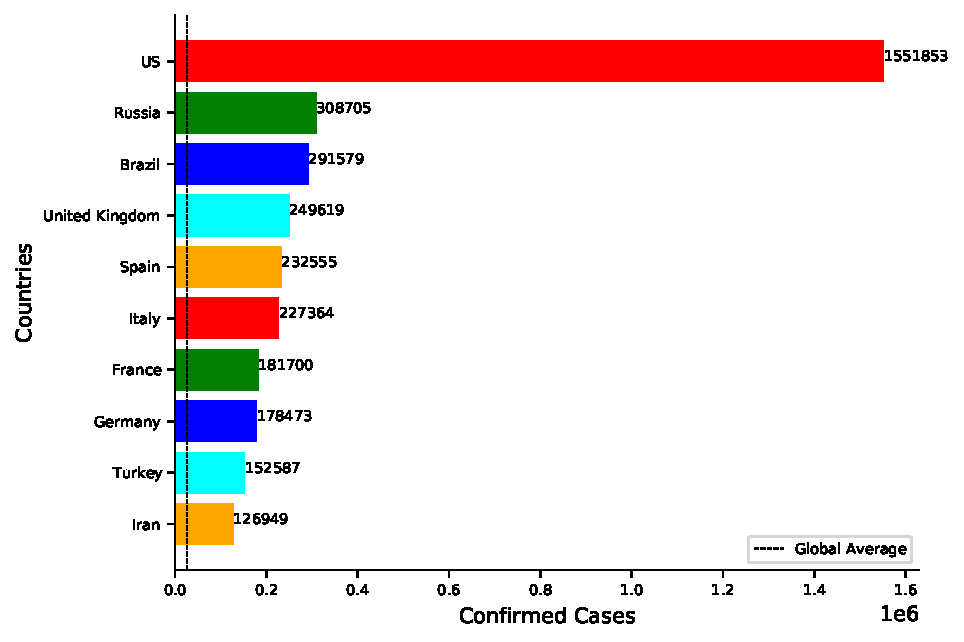
\includegraphics[width=0.5\linewidth]{./images/plot-1.pdf}
	\caption{Number of Confirmed Cases}
	\label{plot_confirmedcases}
\end{figure}

As can be seen in figure \ref{plot_confirmedcases} the number of confirmed cases in these ten countries exceed the global average. Even among the worst hit countries the number of cases in USA is exceptionally high. Number of confirmed cases is USA, which is at first place is ~10.752 times higher than Germany which is at the tenth place. There also exists a huge difference between USA and Brazil, which is at second place. USA has ~2.589 times more cases as that of Brazil. This goes on to reflect that the spread of Coronavirus in USA has a completly different magnitude than the rest of the world. 

\begin{figure}[H]
	\centering
	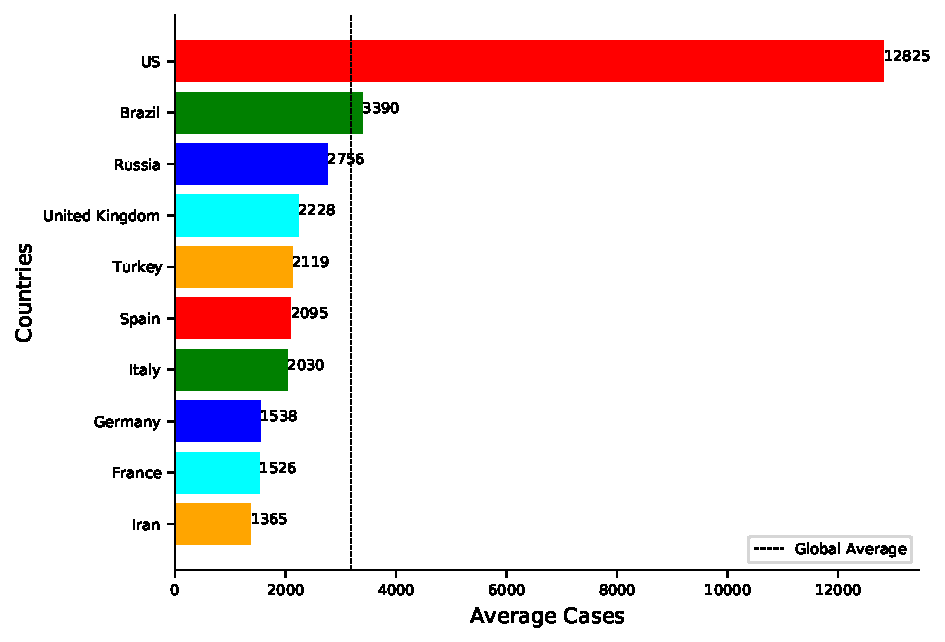
\includegraphics[width=0.5\linewidth]{./images/plot-2.pdf}
	\caption{Number of Confirmed Cases}
	\label{plot_averagecases}
\end{figure}

As mentioned in the previous section, that number of confirmed cases could be an elusive parameter. A country having higher number of confirmed cases might come across as having a more dire situation than a country which has lower number of confirmed cases. However, since infectious diseases follows an exponential curve hence the number of confirmed cases climb very quickly to higher numbers, hence normalizing the total number of cases with the duration can give an indirect insight into the growth rate of confirmed cases.
\\
\\
As can be observed from figure \ref{plot_averagecases}, USA has the highest average number of cases among the worst hit countries. USA and Brazil are the only countries where average number of confirmed cases is higher than the global average. If we compare figure \ref{plot_confirmedcases} and figure \ref{plot_averagecases}, we can observe even though India has higher number of confirmed cases, average cases in India are still lower than Peru, this indicates that Peru has a more aggressive growth rate than India.This analogy can be applied to other countries as well. In Europe the first major outbreak was in Italy, which has seventh highest number of confirmed cases, ranks eight in terms of average cases. France and Germany are the only countries which has the ninth and tenth rank in terms of confirmed cases and and also have the same standing in terms of average number of cases.

\begin{figure}[H]
	\centering
	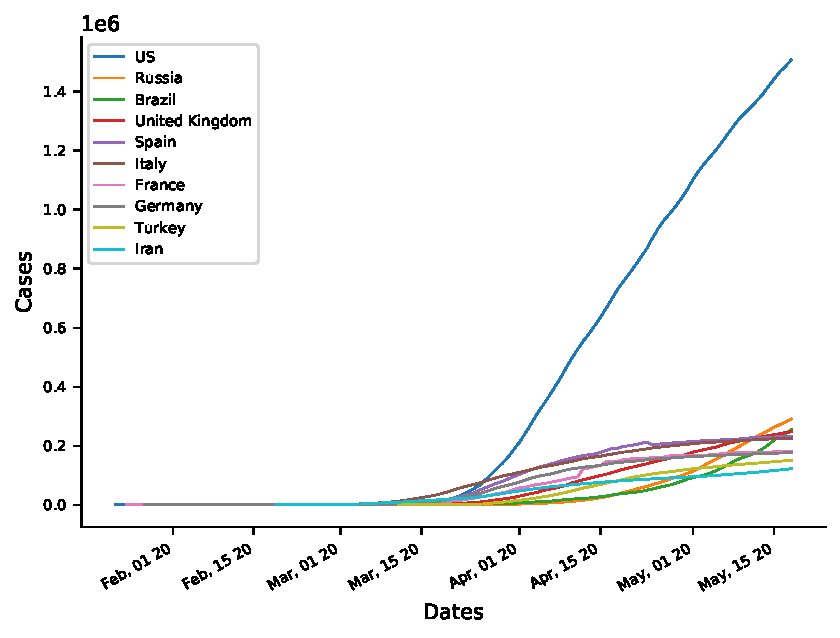
\includegraphics[width=0.5\linewidth]{./images/plot-3.pdf}
	\caption{Number of Confirmed Cases over time}
	\label{plot_caseprogression}
\end{figure}

In order to paint a more clear picture of the spread of infection, rise in the number of confirmed cases needs to be studied. From figure \ref{plot_caseprogression} we can observe that USA and Italy had same number of cases between March and April, but the spread of Coronavirus is much more aggressive in USA than in Itlay. Brazil and Russia had the same number of cases between mid April and May, But Russia had a more agressive growth rate at this point of time hence as a result it developed more cases than Brazil. However Brazil ended up having more cases than Russia as between May and June, the spread of infection became more aggressive in Brazil than in Russia. A sudden spike in the number of cases can be observed for France between April and May. A similar pattern can be observed for Spain, where a small sharp decline can be observed  for Spain, between April and May, this could be attributed to error in reporting or testing. India had the same amount of cases as Peru between May and June, but near the end of June India overtook France, Germany, Italy and Spain.
\\
\\
\begin{figure}[H]
	\centering
	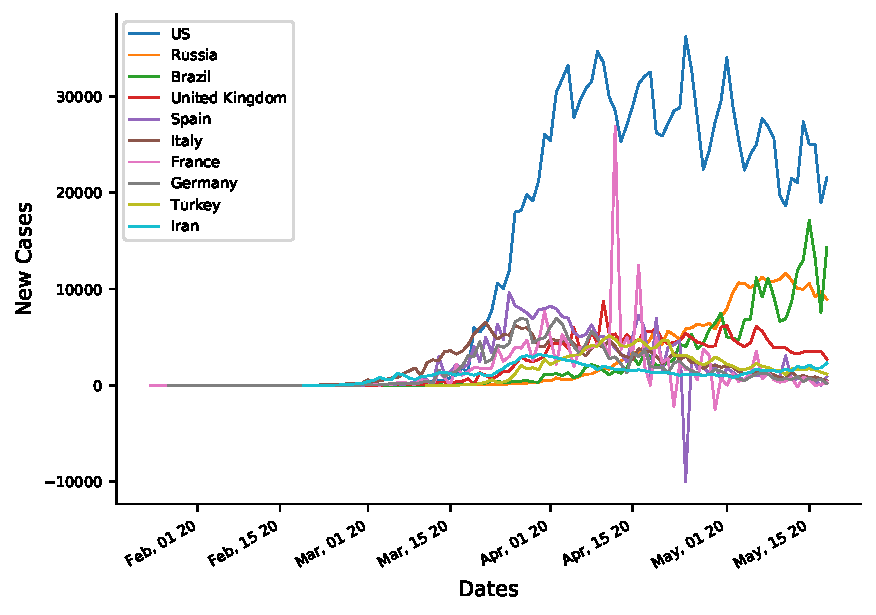
\includegraphics[width=0.5\linewidth]{./images/plot-4.pdf}
	\caption{Number of New Cases over time}
	\label{plot_newcases}
\end{figure}

As it has been mentioned before that total number of cases do not give a complete perspective of the situation. Hence, proceeding further, number of new cases will be studied to better understand the rate of spread of Coronavirus. As can be seen from figure \ref{plot_newcases}, occurrence of new cases in USA spiked after mid-March, a steep rise in new cases can be seen from mid of March till starting of April. 
This trend discontinued after April 1 and the pattern became more irregular. After April 1, several crests and troughs can be observed, even though the pattern seems to be irregular, but on a closer observation it can be seen that after March 15, the crests peak out to lower values and troughs fall to lower values, indicating a possible decline in the number of new cases. This could be an indicator that the measures taken to stop the spread of the Coronavirus are working.
\\
\\
Except for Spain, UK, Italy and Germany, no other country reported less than 10000 cases in a single day. France has reported abrupt increase in the number of new cases which can be observed in the form of huge  spikes. All the countries except USA, Brazil, India and Peru show a similar pattern in which the occurance of new cases increases before decreasing. This is indicative of the fact that the measures taken to curb the spread of Coronavirus are working. We can also observe a peculiar feature in figure \ref{plot_caseprogression}, Spain seems to have negitive number of new cases this is not physically possible. As mentioned above, this might be due to erroneous reporting or erroneous testing.

\begin{figure}[H]
	\centering
	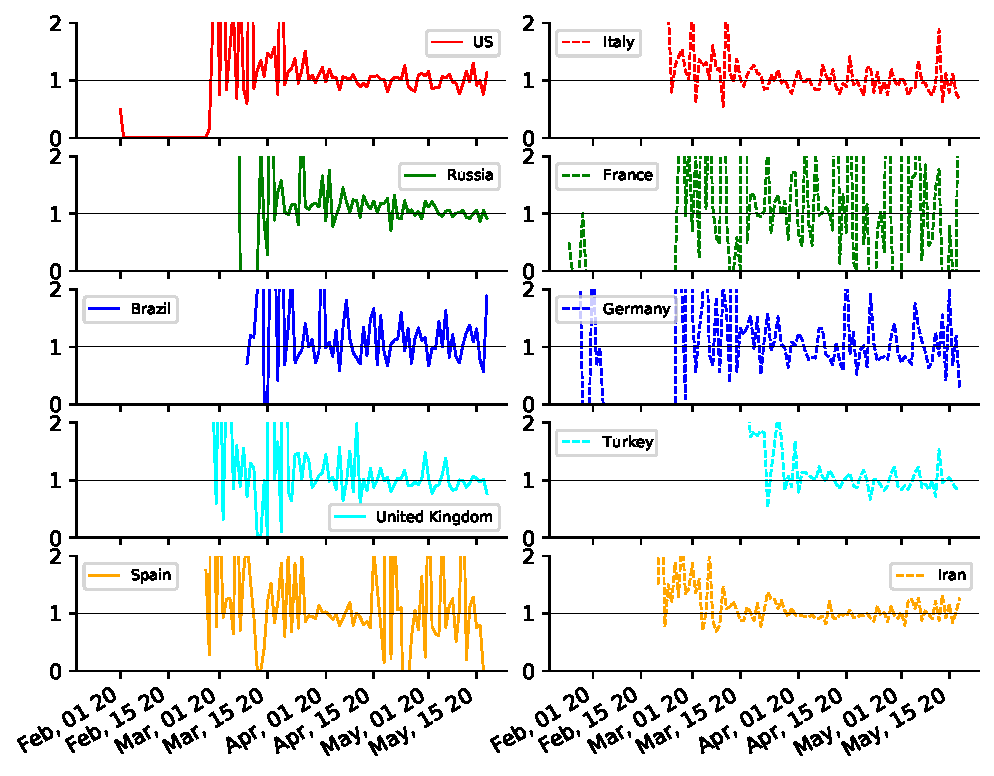
\includegraphics[width=0.5\linewidth]{./images/plot-6.pdf}
	\caption{Growth Rate over time}
	\label{plot_growthrate}
\end{figure}

As was mentioned in the previous section of this report, growth rate could be the best indicator of the situation. The plot originally generated had huge spikes which made it difficult to focus on the important range (0 to 1) of the growth rate. Hence the maximum values of Growth rate was capped to 2 and data for each country was plotted separately.
\\
\\
As we can observe from figure \ref{plot_growthrate}, none of the country has managed to lower the Growth Rate below the critical value of 1. Oscillations close to the critical value can be observed for USA and Russia. Even though USA had the maximum number of confirmed cases, the growth rate observed after April 1 has dramatically decreased and oscillates very close to 1. Similar behavior can be seen with Russia after May 1. It can be observed that after May 1, variation in Growth Rate around the critical value is pronounced in USA than in Russia.Both India has also managed to keep the Growth Rate close to critical value after May 1.

\begin{figure}[H]
	\centering
	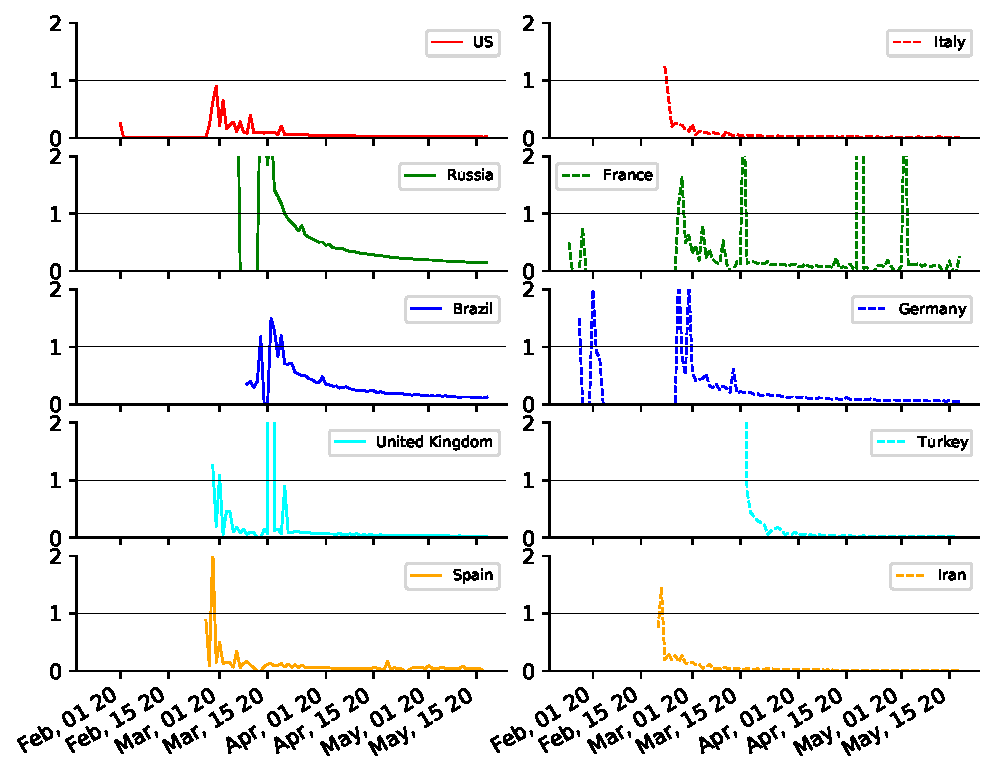
\includegraphics[width=0.5\linewidth]{./images/plot-7.pdf}
	\caption{Moving Average of Growth Rate over time}
	\label{plot_growthrateMA}
\end{figure}    

As can be seen from figure \ref{plot_growthrateMA}, moving averages have eliminated irregularities when applied to growth rate. USA and India are the only countries which has managed to keep the moving average below the critical value of 1. Although moving average eventually falls below 1 for all the countries, it can be observed that all the countries except India and USA have spikes in the moving average of Growth Rate which cross the critical value of 1.

\section{Conclusion}

Based on the observations made in previous section, following conclusions can be drawn:
\begin{itemize}
	\item Coronavirus is highly contagious and the number of new cases can increase extreamly rapidly as seen in the case of USA.
	\item Number of occurrence of new cases is a very strong indicator of evaluating the situation within a country
	\item Tracking the number of new cases could give an insight of the situation, but growth rate could be a better indicator that provides more conclusive analysis
	\item  A drop in the number of new cases could be observed for some countries, this indicates that preventative measures such as lock-downs are actually effective in preventing the spread of Coronavirus  
\end{itemize}  

\bibliographystyle{ieeetr}
\bibliography{myrefrences}

\end{document}